% !TeX encoding = UTF-8
% !TeX program = xelatex

\documentclass{cjc}

\usepackage{booktabs}
\usepackage{graphicx}
\usepackage{siunitx}
\usepackage{array}

\classsetup{
  title        = {GRAF-Mem：面向长时具身问答的图增强检索与主动记忆维护方法},
  title*       = {GRAF-Mem: Graph-Augmented Retrieval and Active Memory Maintenance for Long-Horizon Embodied Question Answering},
  short-title  = {GRAF-Mem：图增强检索与主动记忆维护},
  authors      = {
    author1 = {
      name         = {刘谨旗},
      name*        = {Jinqi Liu},
      affiliations = {aff1},
      biography    = {男，本科生，主要研究领域为具身智能、长期情景记忆和大语言模型智能体.},
      biography*   = {Undergraduate student. His research interests include embodied intelligence, long-term episodic memory, and large language model agents.},
      email        = {jeankey82704@mail.nwpu.edu.cn},
    },
  },
  affiliations = {
    aff1 = {
      name  = {西北工业大学 软件学院，西安 710072},
      name* = {School of Software, Northwestern Polytechnical University, Xi'an 710072, China},
    },
  },
  abstract     = {
    长期服务机器人需要在持续交互中记录任务执行、物体状态和失败原因，并回答后续回溯性问题。
    现有长上下文、检索增强和层级记忆方法难以同时解决跨事件证据召回不足、存储规模膨胀和错误记忆修正困难等问题。
    为此，本文提出 GRAF-Mem，一种面向长时具身问答的图增强检索与主动记忆维护框架。
    该方法在层级记忆树之上构建事件关联图，将时间、物体、位置、动作和因果关系统一用于检索、遗忘和修正。
    在 TEACh 长历史问答实验中，GRAF-Mem 在 $|h|=100$ 设置下达到 49.0\% 语义完全正确率和 75.0\% 至少部分正确率，相比 H-EMV 参考基线将平均 token 开销降低 78.0\%。
    遗忘实验表明，激进配置可减少 31.70\% 的序列化记忆树大小和 50.83\% 的关系数量；受控错误注入实验验证了从用户反馈到后续答案改善的闭环修正能力。
  },
  abstract*    = {
    Long-term service robots need to record task executions, object states, and failure causes, and answer later questions about their experiences.
    Existing long-context, retrieval-augmented, and hierarchical memory methods still struggle with cross-event evidence recall, storage growth, and erroneous memory correction.
    This paper proposes GRAF-Mem, a graph-augmented retrieval and active memory maintenance framework for long-horizon embodied question answering.
    GRAF-Mem builds an event association graph over a hierarchical memory tree and uses temporal, object, spatial, action, and causal relations for retrieval, forgetting, and correction.
    On TEACh long-history question answering, GRAF-Mem achieves 49.0\% semantic correctness and 75.0\% partial correctness under $|h|=100$, while reducing average token cost by 78.0\% compared with the H-EMV reference baseline.
    The aggressive forgetting setting reduces serialized memory size by 31.70\% and relation count by 50.83\%, and controlled error injection verifies the correction loop from user feedback to improved future answers.
  },
  keywords     = {长期情景记忆, 具身问答, 图增强检索, 记忆遗忘, 记忆修正},
  keywords*    = {long-term episodic memory, embodied question answering, graph-augmented retrieval, memory forgetting, memory correction},
  doi           = {},
}

\setlength{\headheight}{27.2pt}

\usepackage{hyperref}

\begin{document}

\maketitle

\section{引言}

近年来，大语言模型、多模态感知和服务机器人技术快速发展，机器人正逐渐从短时任务执行走向家庭服务、医疗辅助和人机协作等长期开放场景\cite{siciliano2016robotics,vaswani2017attention,brown2020gpt3,achiam2023gpt4,reid2024gemini}。
在这类场景中，机器人不仅需要完成当前指令，还需要持续记录自身经历，并回答“上周完成了什么任务”“某个物体曾经放在哪里”“任务失败前发生了什么”等回溯性问题。
将机器人历史经历组织为可检索、可问答的自然语言记忆，是提升长期人机交互可信度和可解释性的重要基础。
这一能力与情景记忆语言化密切相关，即把智能体过去的事件及其上下文转化为可查询、可表达的记忆结构\cite{tulving1972episodic,barmann2025episodic}。
与一次性任务不同，长期具身问答的核心难点不在于单个场景是否能被理解，而在于系统能否在大量历史事件之间建立可追溯的联系。
例如，同一个杯子可能先后出现在取物、清洗和放置三个任务中；一次失败动作的原因可能位于前一段交互中；用户后续纠正的事实也可能已经被多个高层摘要引用。
因此，一个面向长期服务机器人的记忆系统既要能“记住”，也要能在长期运行中持续整理、筛选和修正记忆。

围绕长历史问答，现有研究大致形成了三类路线。
第一类方法直接利用长上下文语言模型处理完整历史\cite{brown2020gpt3,achiam2023gpt4,gemini2023gemini,reid2024gemini}，实现简单，但推理成本随历史长度快速增长，且长序列中部信息容易被忽略\cite{liu2024lost}。
第二类方法采用检索增强生成，通过向量检索选择少量相关片段后再生成答案\cite{lewis2020rag,karpukhin2020dpr,reimers2019sbert,johnson2019faiss,nogueira2019reranking,gao2023hyde}，能够降低上下文开销，但通常把记忆片段视为相互独立的文本块，难以利用事件之间的时间、物体和空间关联。
第三类方法将长期经历组织为层级摘要树，并使用大语言模型智能体逐层检索\cite{barmann2025episodic,plewnia2025combining}。
层级结构有利于压缩长历史，但树结构主要表达纵向父子关系，对跨任务、跨时间的横向证据发现支持不足。

长期机器人记忆还面临与普通文本问答不同的维护需求。
如图\ref{fig:framework}所示，机器人历史由多模态感知、动作轨迹、场景图、用户语音和层级摘要共同构成。
在长期部署中，系统需要面对三个具体挑战。
第一，相关证据往往分散在不同任务和不同树分支中，仅依赖文本相似度或树导航容易漏召回。
第二，原始图像、音频、场景关系和事件摘要会随着运行时间持续增长，如果全部完整保存，将造成不可忽视的存储压力。
第三，视觉识别、语音转写或语言摘要中的错误一旦写入记忆，就可能在层级摘要和后续问答中传播。
因此，长期情景记忆不应只是被动的历史保存结构，还应具备检索、压缩和修正的主动维护能力。
本文将这三个问题视为同一长期记忆生命周期中的不同阶段：检索决定系统如何使用已有记忆，遗忘决定系统如何在预算内保留记忆，修正决定系统如何在发现错误后更新记忆视图。
若三者分别由互不相干的模块处理，系统容易出现检索依赖的关系被遗忘破坏、修正后的事实无法被重新召回等问题。
因此，本文尝试用统一的事件关联图连接三个阶段，使其共享同一组事件关系和结构重要性信号。

为解决上述问题，本文提出 GRAF-Mem，一种面向长时具身问答的图增强检索与主动记忆维护框架；其中 GRAF-Mem 表示 Graph Augmented Retrieval and Adaptive Forgetting Memory，即图增强检索与自适应遗忘记忆。
GRAF-Mem 保留层级记忆树作为基础存储结构，同时在事件级节点之间构建事件关联图。
该图在检索阶段提供横向扩展路径，在遗忘阶段提供结构重要性信号，在修正阶段提供传播检测依据。
通过这种统一的图结构，本文将原本相对分离的证据检索、存储压缩和错误维护问题纳入同一框架。

本文的主要贡献如下：
\begin{itemize}
  \item 问题层面：本文面向长期服务机器人情景记忆问答，系统研究长历史检索效率、记忆存储膨胀和错误记忆修正三个相互关联的问题。
  \item 方法层面：本文提出事件关联图增强检索方法、效用引导的渐进式遗忘策略和反馈驱动的非侵入式记忆修正机制，形成一个可检索、可压缩、可修正的主动记忆框架。
  \item 实验层面：本文在 TEACh 长历史问答和 ARMARX 真实机器人记忆切片上进行验证，结果表明 GRAF-Mem 能提升问答正确率、降低 token 开销，并在可控语义退化下实现存储压缩和错误修正。
\end{itemize}

\section{相关工作}

\subsection{机器人情景记忆}

情景记忆最早源于认知科学，用于描述个体对过去事件及其上下文的记忆能力\cite{tulving1972episodic}。
在机器人领域，情景记忆通常用于记录感知、动作和交互历史，从而支持后续问答、解释和任务规划。
早期方法包括隐向量记忆、符号化知识库和自然语言记忆三类。
隐向量方法借助神经网络表示或注意力机制压缩经历\cite{bahdanau2015attention,rothfuss2018deep}，但语义不可直接检查。
符号化方法如 KnowRob 和 RoboEarth 具有较强可解释性\cite{tenorth2009knowrob,waibel2011roboearth}，但本体和规则维护成本较高。
自然语言记忆方法利用大语言模型的语义理解能力组织机器人经历\cite{rosenthal2016verbalization,zhu2017autonomous,barmann2021deep,liu2023reflect,barmann2025episodic}，更适合开放环境中的长期问答。
本文基于自然语言层级记忆结构，进一步关注跨事件关联和长期维护。
表\ref{tab:memorycompare}从表示形式、检索方式和可维护性三个角度比较了三类路线。
可以看出，隐向量方法和符号化方法分别偏重效率与精确性，但都难以同时满足开放环境中的可解释问答和长期维护需求。
自然语言记忆更适合与大语言模型结合，但若缺少结构化索引和维护机制，也容易退化为不断追加的文本日志。
GRAF-Mem 的定位正是在自然语言层级记忆基础上加入图结构与主动维护能力。

\begin{table*}[t]
  \centering
  \caption{机器人情景记忆方法对比}
  \label{tab:memorycompare}
  \small
  \begin{tabular}{@{}p{2.1cm}p{3.1cm}p{3.0cm}p{1.8cm}p{2.1cm}p{2.0cm}@{}}
    \toprule
    方法类型 & 记忆表示 & 检索方式 & 可解释性 & 泛化性 & 可维护性 \\
    \midrule
    隐向量方法 & 固定维度潜在向量 & 向量相似度或策略网络内部状态 & 较低 & 依赖训练分布 & 较弱 \\
    符号存储方法 & 本体、谓词、关系图谱 & 规则推理或数据库查询 & 较高 & 依赖人工本体 & 中等 \\
    自然语言记忆 & 文本摘要 & LLM Agent 检索与问答 & 较高 & 利用预训练模型 & 需要额外维护机制 \\
    GRAF-Mem & 层级树 + 事件关联图 & 语义检索、图扩展与结构化工具 & 较高 & 面向开放历史 & 支持遗忘与修正 \\
    \bottomrule
  \end{tabular}
\end{table*}

\subsection{长历史检索与图增强方法}

检索增强生成是长上下文问答中的主流范式之一\cite{lewis2020rag}。
典型组件包括稠密检索\cite{karpukhin2020dpr}、句向量表示\cite{reimers2019sbert}、向量索引\cite{johnson2019faiss}、查询扩展\cite{gao2023hyde}和重排序\cite{nogueira2019reranking}。
近年来，研究者进一步将树和图结构引入长文档或长视频检索，例如 RAPTOR\cite{sarthi2024raptor}、Graph RAG\cite{edge2024graphrag}、VideoTree\cite{wang2024videotree}和 VideoAgent\cite{wang2024videoagent}。
长视频问答和第一人称记忆问答也提供了相近的问题背景\cite{barmann2022egocentric}。
与普通文档不同，机器人经历包含显式的时间顺序、物体实例、动作状态和空间关系。
因此，本文直接从机器人事件节点构建关联图，而不是仅对文本片段做离线聚类。

\subsection{长期记忆管理与修正}

长期记忆管理与认知科学中的遗忘曲线和系统巩固理论密切相关\cite{ebbinghaus1913memory,winocur2011memory}。
在大语言模型系统中，MemGPT、LongMem、MemWalker 和 Generative Agents 等工作探索了长对话或长文本中的记忆管理\cite{packer2023memgpt,wang2023longmem,chen2023memwalker,park2023generative}。
这些方法主要管理文本上下文，而机器人记忆还包含原始多模态文件、场景图和层级摘要。
在错误修正方面，知识编辑方法如 ROME、MEMIT 和 Fast Model Editing 主要修改模型参数中的事实关联\cite{meng2022rome,meng2023memit,mitchell2022fast,mitchell2022memory}，强化学习和人类反馈也可用于策略优化\cite{christiano2017rlhf}。
然而，机器人长期记忆中的错误往往存在于外部记忆数据本身。
因此，本文选择在记忆视图层修正错误摘要，而不直接修改语言模型参数。

\section{预备知识}

\subsection{问题定义}

设机器人在长期运行中形成一段历史 $H=\{E_1,E_2,\ldots,E_N\}$，其中每个事件 $E_i$ 包含时间范围、动作、场景图、物体集合、用户语音和自然语言摘要等信息。
层级情景记忆将这些事件组织为一棵树 $\mathcal{T}$，底层节点保存细粒度多模态数据，高层节点保存跨事件摘要。
给定用户问题 $q$，系统需要从 $\mathcal{T}$ 中检索证据集合 $C(q)$，并生成答案 $a$。
长期部署条件下，系统还需要在存储预算 $B$ 内维护记忆，同时在收到反馈 $f=(q,a_{\mathrm{wrong}},a_{\mathrm{correct}})$ 后修正错误记忆。

因此，本文研究的问题可以概括为：在不破坏层级记忆树原始结构的前提下，如何构建一种外部维护机制，使系统能够高效检索相关证据、选择性压缩低价值记忆，并根据反馈修正错误事实。

\subsection{层级情景记忆结构}

\begin{figure}[t]
  \centering
  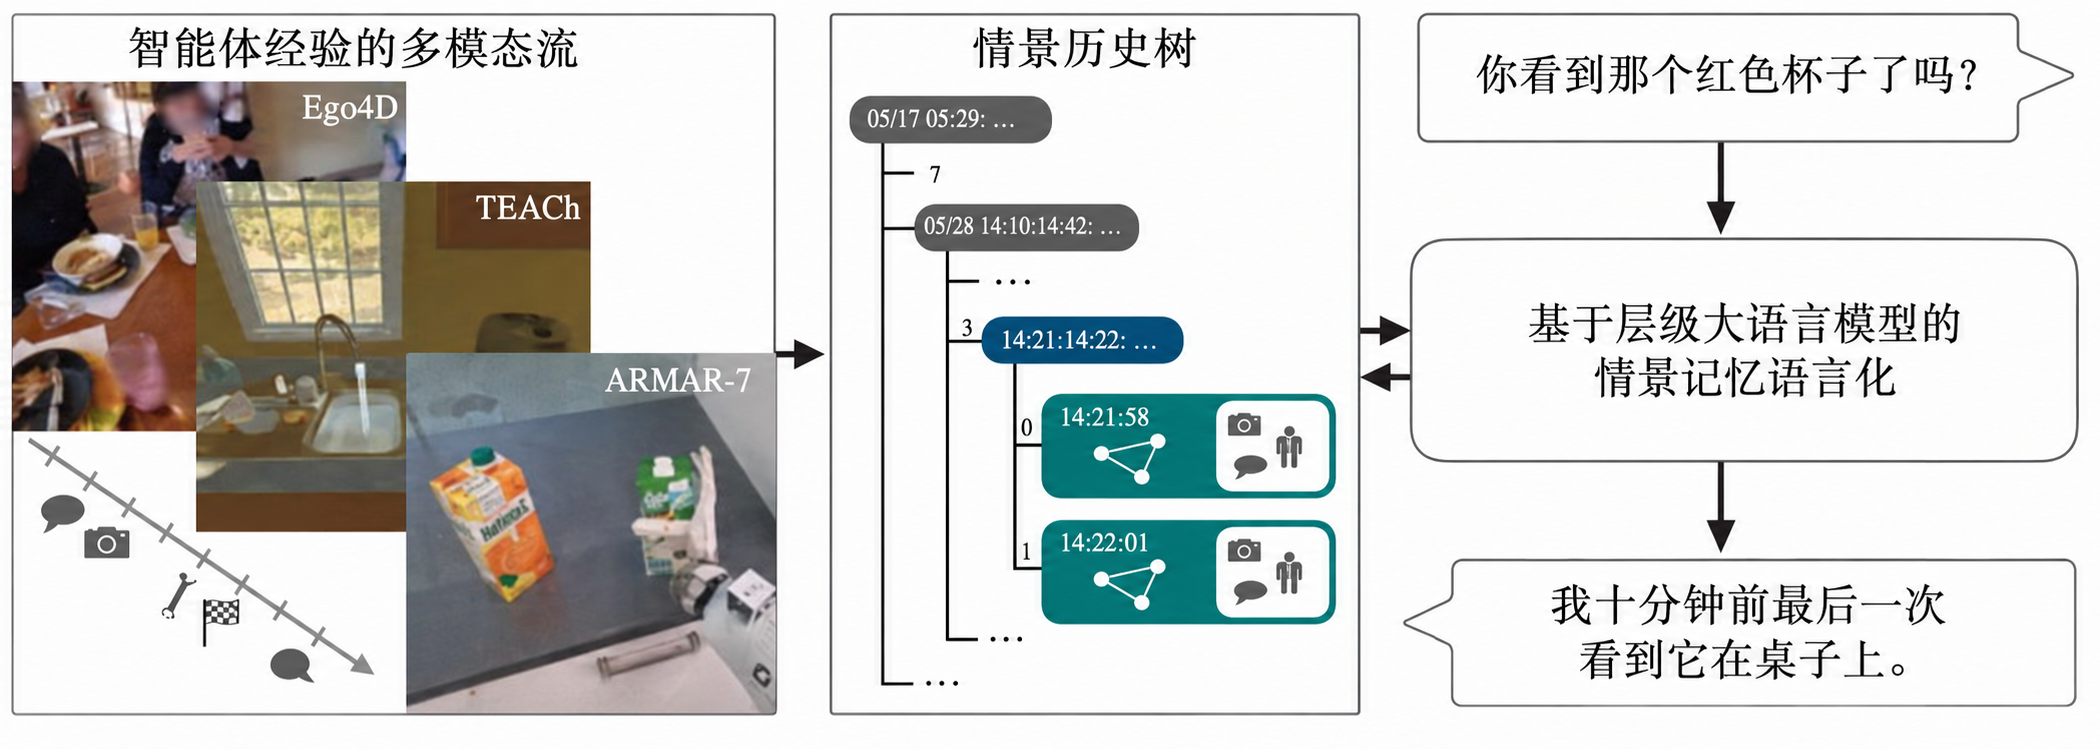
\includegraphics[width=.92\linewidth]{../content/figures/图2-2 层级情景记忆树表示.png}
  \caption{层级情景记忆树表示。底层保存原始多模态感知与场景图，高层保存事件、目标和长期摘要。}
  \label{fig:memorytree}
\end{figure}

本文以层级情景记忆树作为基础存储结构，如图\ref{fig:memorytree}所示。
底层 L0 节点保存图像、音频等原始感知数据；L1 节点保存场景图中的物体、属性和空间关系；L2 节点对应细粒度事件或动作摘要；L3 节点概括一个目标或任务片段；更高层节点继续聚合跨任务、跨日期的长期摘要。
这种结构具有两个优点：一是不同层级分别对应不同粒度的问答需求，既能支持局部细节查询，也能支持任务概览查询；二是自然语言摘要便于大语言模型智能体读取和推理。
但层级树主要表达父子关系，一条事件只能通过其祖先和子孙与其他事件相连。
对于“同一物体后来还出现在哪里”“某个动作失败前后发生了什么”等横向问题，仅依赖树结构会造成检索路径过长或证据遗漏。
因此，GRAF-Mem 在不改变原始树的前提下额外构建事件关联图，将 L2 事件节点之间的横向关系作为外部索引层。

\subsection{系统框架}

\begin{figure}[t]
  \centering
  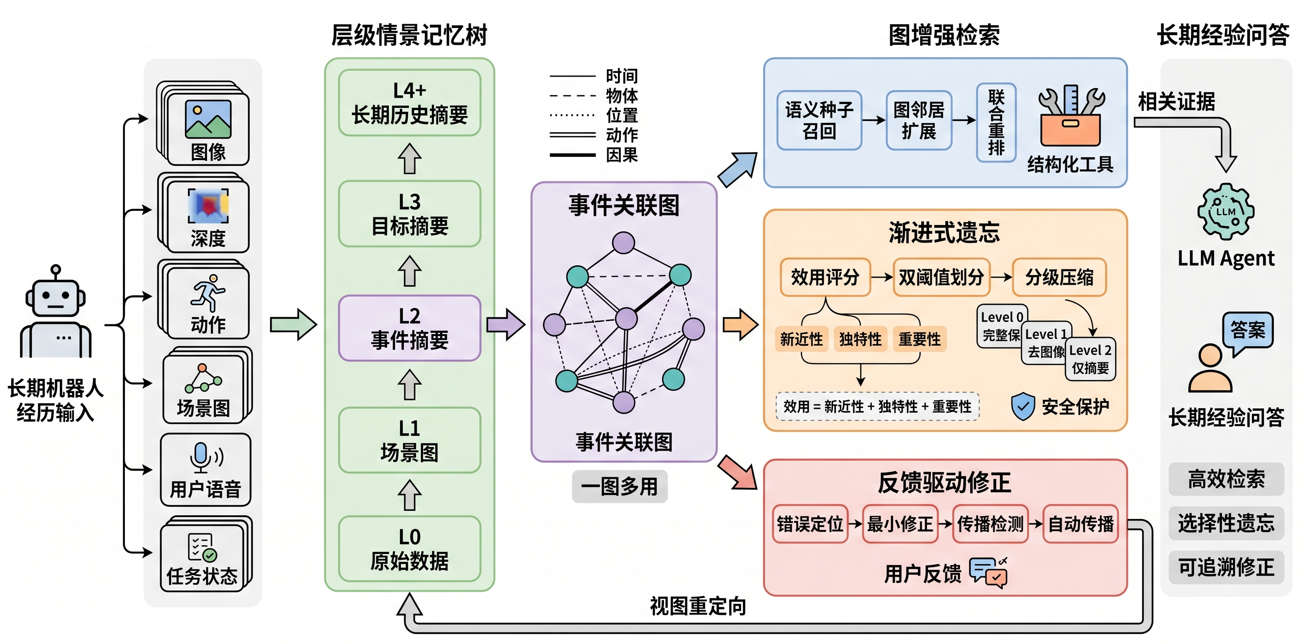
\includegraphics[width=.95\linewidth]{../content/figures/图1-2 GRAF-Mem总体框架图.png}
  \caption{GRAF-Mem总体框架。系统在层级记忆树之上构建事件关联图，并将其用于图增强检索、渐进式遗忘和反馈驱动修正。}
  \label{fig:framework}
\end{figure}

GRAF-Mem 的整体框架如图\ref{fig:framework}所示。
系统首先从层级记忆树中的事件级节点派生事件关联图，并为每个事件保留回指原始树节点的引用。
在问答阶段，图结构与结构化工具共同引导智能体检索相关证据。
在记忆维护阶段，系统根据事件效用执行不同等级的压缩，并使用反馈驱动修正模块对错误摘要进行非侵入式覆盖。
三个模块共享同一事件图，使图结构成为贯穿长期记忆检索和维护的统一索引。

\section{方法}

\subsection{事件关联图构建}

事件关联图以 L2 事件摘要节点为图节点。
对每个事件 $E_i$，系统提取物体实例集合 $O(E_i)$、动作标签 $A(E_i)$、位置签名 $P(E_i)$和时间范围 $T(E_i)$。
在此基础上构建五类边。
时间相邻边连接同一目标下前后相邻的事件。
共享物体边连接具有共同物体实例的事件，边权为物体集合的 Jaccard 相似度。
共位置边连接位置签名相似的事件，位置签名由场景中的大型固定物体近似表示。
相似动作边连接动作模板语义相似的事件，动作中的具体对象编号会先被归一化。
因果边用于连接可能存在失败传播或因果关系的事件，在主实验中作为可选边类型。
选择 L2 事件作为图节点，主要是因为 L2 是树结构中最细粒度的自然语言层，既保留了具体动作和局部场景信息，又不会像原始帧一样规模过大。
在 $|h|=50$ 的长历史设置下，一段历史通常包含约 5000--6000 个 L2 节点，能够在可接受成本内完成连边和缓存。

共享物体边的权重采用 Jaccard 相似度：
\begin{equation}
w_o(E_i,E_j)=\frac{|O(E_i)\cap O(E_j)|}{|O(E_i)\cup O(E_j)|}.
\label{eq:objectedge}
\end{equation}
共位置边同样采用位置签名集合的 Jaccard 相似度，其中位置签名由 Sink、Fridge、CounterTop、Cabinet 等大型固定物体近似表示。
相似动作边先将包含具体对象编号的动作归一为动作模板，再用句向量计算动作模板间相似度，从而把计算规模由事件两两比较降低为动作模板两两比较。
时间相邻边和共享物体边是零 LLM 成本的规则边，因果边需要额外推理，故主实验默认不启用。

为避免图过密，系统对高频无信息物体进行过滤，并对每个节点在每类边上仅保留权重最高的若干邻居。
图构建结果通过历史内容签名缓存，同一段长历史在多次评测中可直接复用。
这一图结构不仅服务于检索，也在后续遗忘和修正模块中被复用。
具体而言，遗忘模块利用轻量图度中心性判断哪些事件是结构枢纽；修正模块则沿时间邻居和树结构邻域检测错误传播。
由此，事件关联图不只是一个检索加速器，而是长期记忆主动维护的统一结构基础。

\subsection{图增强检索与结构化工具}

当用户提出问题 $q$ 时，GRAF-Mem 执行三阶段检索。
第一阶段为语义种子召回，使用句向量模型计算问题与记忆节点可检索文本之间的相似度，得到种子集合 $S_0$。
第二阶段为图邻居扩展，根据问题中的时间词、物体名、空间词和因果词激活不同边类型，从 $S_0$ 沿图扩展得到候选集合 $S_1$。
第三阶段将 $S_0$ 和 $S_1$ 合并，并按式(\ref{eq:rerank})重排：
\begin{equation}
\mathrm{score}(q,n)=
\alpha \mathrm{sim}(q,n)+
\beta \mathrm{graph}(q,n)+
\gamma \mathrm{depth}(n),
\label{eq:rerank}
\end{equation}
其中 $\mathrm{sim}(q,n)$ 表示节点自身与问题的语义相似度，$\mathrm{graph}(q,n)$ 表示活跃图邻居的加权贡献，$\mathrm{depth}(n)$ 表示层级深度先验。
默认权重为 $\alpha=0.70$、$\beta=0.25$、$\gamma=0.05$，以保证语义相关性仍占主导，同时引入图结构信号。
查询意图路由器根据问题词触发不同边类型：包含“之前/之后”等时间线索时优先启用时间相邻边，包含具体物体名时启用共享物体边，包含“在哪里”等空间线索时启用共位置边，包含“为什么/失败”等词时启用因果边。
若未命中明确规则，则默认启用时间、物体、位置和动作四类边，以保证一般问题也能获得横向证据补充。

除图增强搜索外，系统还提供七类结构化检索工具，覆盖任务列表、任务查找、物体查找、日期查找、事件日期查找、时间邻居查找和动作查找。
这些工具将任务、物体、日期和时间邻居查询转化为确定性或半确定性查找，减少智能体在长历史树中的自由展开次数。
这些工具均直接读取层级树中的结构化字段，不额外调用大语言模型。
当问题可由工具高置信回答时，智能体可直接生成答案，避免在整棵树上反复展开、折叠和搜索。

\subsection{缓存体系与执行护栏}

长历史评测的稳定性不仅依赖检索算法，还依赖执行层面的约束。
本文设置三类护栏：预处理缓存、checkpoint 容错以及 token 与时间上限。
每段长历史在正式问答前完成层级摘要树、事件图和嵌入向量构建，问答阶段只读缓存，从而把记忆构建成本与单次问答成本分离。
长时间评测中，系统在每个样本完成后写入结果文件，中断后可跳过已完成样本；对于少量瞬时 API 错误，允许有限次数重试。
此外，系统对短对象名和日期表达式设置专门规则，以减少子串误匹配和相对时间解析错误。
这些护栏不直接改变模型能力，但能降低自由搜索引入的额外 token 开销和噪声证据。

\subsection{效用引导的渐进式遗忘}

\begin{figure}[t]
  \centering
  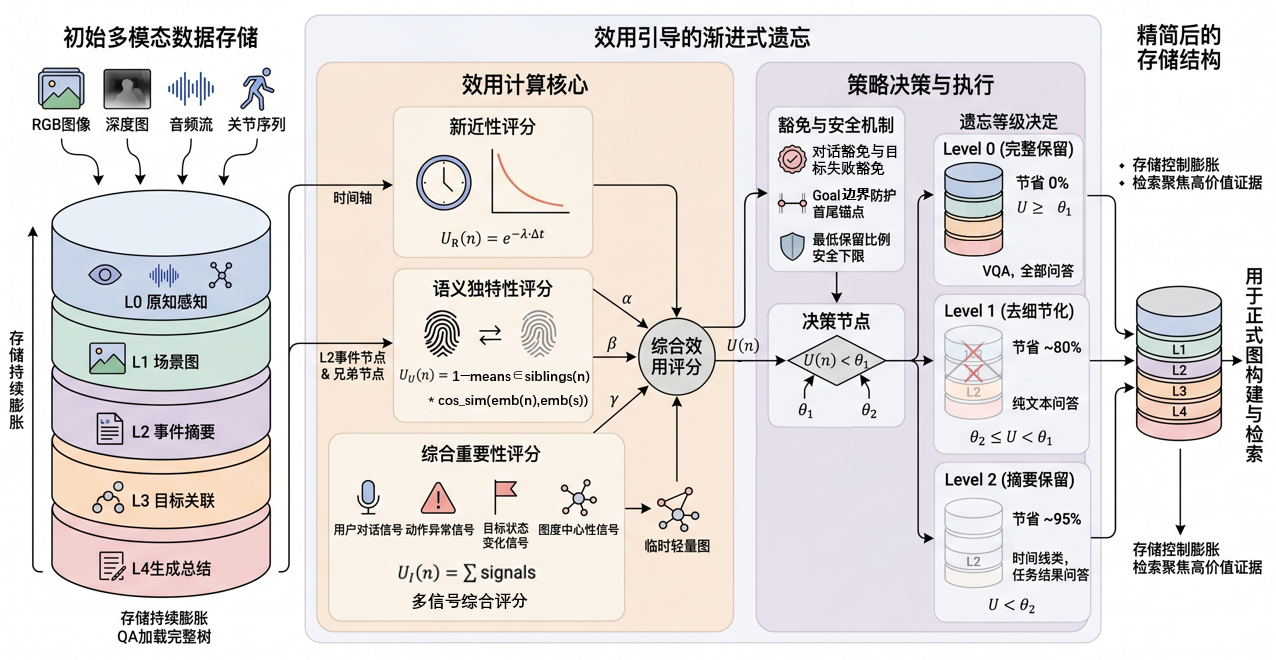
\includegraphics[width=.98\linewidth]{../content/figures/图4-1 效用引导的渐进式遗忘系统架构图.png}
  \caption{效用引导的渐进式遗忘。系统综合新近性、独特性和重要性计算效用，并执行分级压缩。}
  \label{fig:forgetarch}
\end{figure}

为控制长期存储增长，GRAF-Mem 为每个事件节点计算效用分数：
\begin{equation}
U(n)=\alpha R(n)+\beta D(n)+\gamma I(n),
\label{eq:utility}
\end{equation}
其中 $R(n)$ 为新近性，采用指数遗忘曲线建模；$D(n)$ 为语义独特性，定义为节点与兄弟节点平均嵌入相似度的一减值；$I(n)$ 为重要性，由用户对话、动作失败、目标状态变化和轻量图度中心性四类信号组成。
默认权重为 $\alpha=0.3$、$\beta=0.3$、$\gamma=0.4$。
如图\ref{fig:forgetarch}所示，新近性用于刻画近期事件更可能被追问的规律，独特性用于保护同一任务中不可替代的事件，重要性用于保护用户对话、失败动作、目标边界和图结构枢纽。
新近性具体采用
\begin{equation}
R(n)=\exp(-\lambda \Delta t),\quad \lambda=\ln(2)/\mathrm{half\_life},
\label{eq:recency}
\end{equation}
其中 $\Delta t$ 为当前时刻与事件发生时刻的时间间隔。
独特性定义为
\begin{equation}
D(n)=1-\mathrm{mean}_{s\in \mathrm{siblings}(n)}\cos(\mathrm{emb}(n),\mathrm{emb}(s)).
\label{eq:unique}
\end{equation}
若一个事件只是连续导航帧中的重复观察，其独特性较低；若该事件包含用户语音、失败状态或罕见物体状态变化，其独特性会显著升高。

根据 $U(n)$，系统将事件划分为三个保留等级。
Level 0 完整保留所有多模态数据、场景图和摘要。
Level 1 删除原始图像和音频等大对象，但保留场景图文本和摘要。
Level 2 仅保留自然语言摘要和时间戳，用于支持概览类和时间线类问答。
为了降低误删关键证据的风险，系统设置对话豁免、失败豁免、目标边界保护和最低完整保留比例。
因此，遗忘不是简单删除事件，而是按信息价值逐级降低记忆细节。
表\ref{tab:forgetlevels}总结了三种遗忘等级。
这一设计与人类记忆从情景细节逐渐转化为语义要旨的过程相似：重要事件保留多模态细节，普通事件保留结构化文本，低价值重复事件仅保留摘要。

\begin{table*}[t]
  \centering
  \caption{三级渐进式遗忘操作}
  \label{tab:forgetlevels}
  \small
  \begin{tabular}{@{}p{1.4cm}p{2.2cm}p{3.9cm}p{4.0cm}p{2.8cm}@{}}
    \toprule
    等级 & 条件 & 保留内容 & 压缩内容 & 支持的问答类型 \\
    \midrule
    Level 0 & $U\ge\theta_1$ & 原始图像、音频、场景图、摘要与时间戳 & 无 & 全部问题，包括依赖多模态细节的问题 \\
    Level 1 & $\theta_2\le U<\theta_1$ & 场景图文本、物体关系、事件摘要与时间戳 & 删除原始图像和音频 & 主要纯文本和关系类问答 \\
    Level 2 & $U<\theta_2$ & 自然语言摘要和时间戳 & 清空场景图细节和辅助字段 & 概览、时间线和任务结果类问答 \\
    \bottomrule
  \end{tabular}
\end{table*}

\subsection{反馈驱动的记忆修正}

\begin{figure}[t]
  \centering
  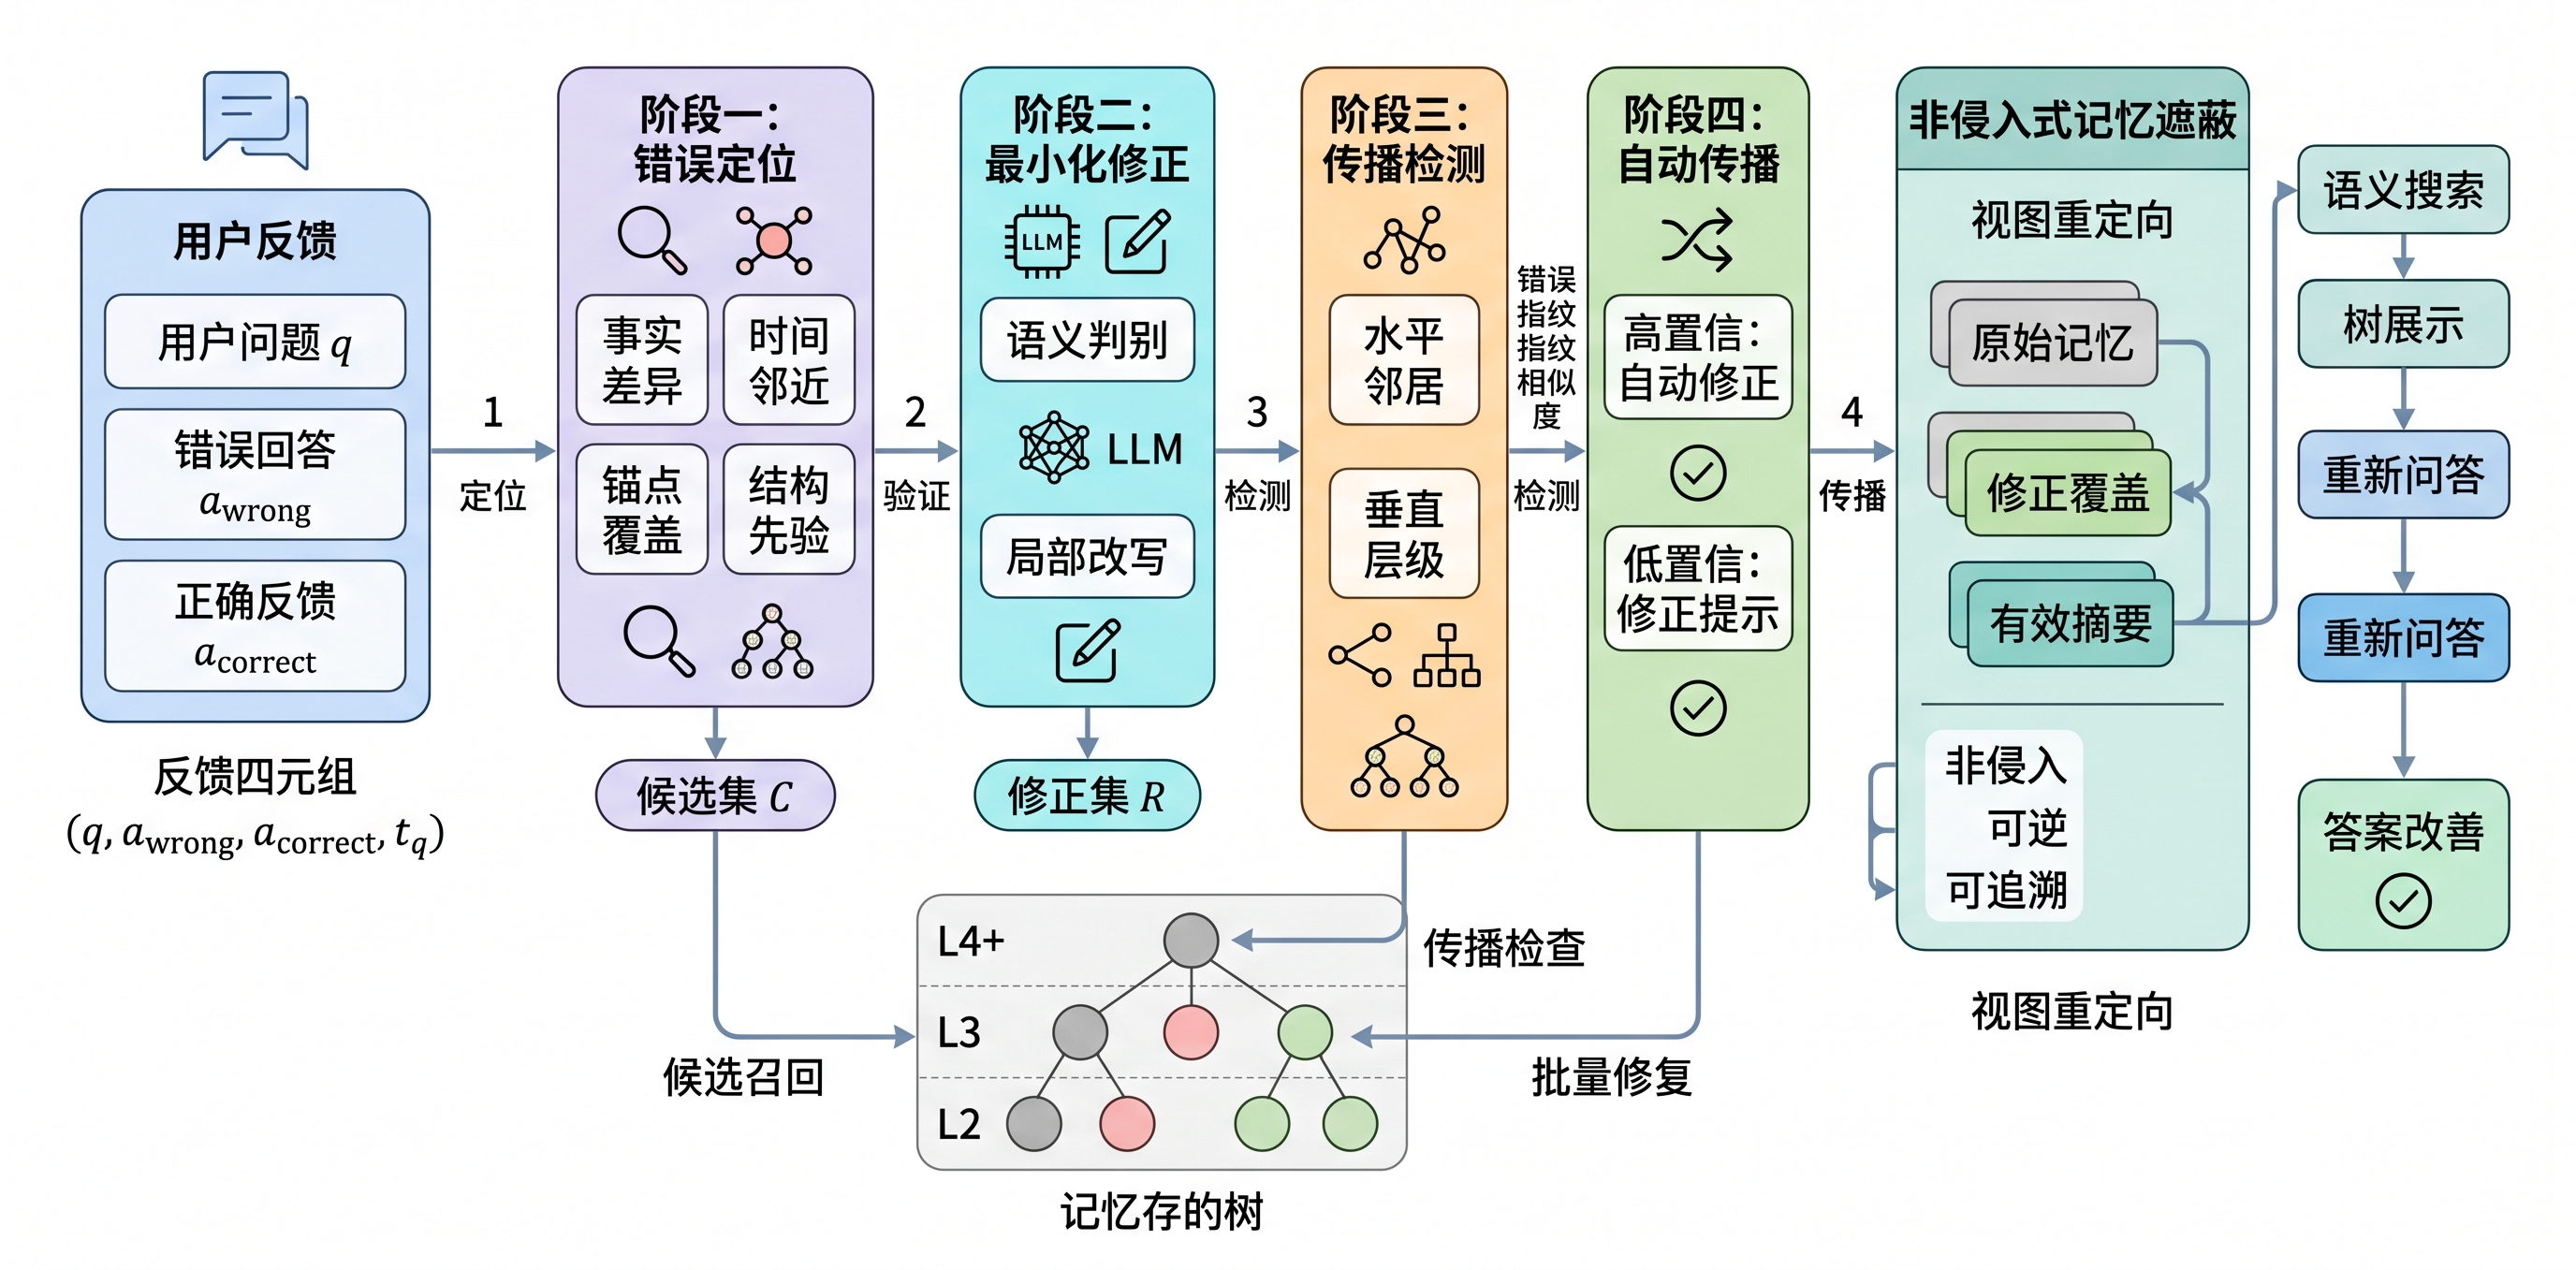
\includegraphics[width=.98\linewidth]{../content/figures/图5-1 反馈驱动记忆修正流程图.png}
  \caption{反馈驱动记忆修正流程。系统先定位候选错误节点，再执行最小化修正和传播检测。}
  \label{fig:correction}
\end{figure}

当用户反馈指出某个回答存在错误时，系统接收 $(q,a_{\mathrm{wrong}},a_{\mathrm{correct}},t_q)$，并抽取实体、关系、错误值和正确值构成纠错线索。
修正过程包含四个阶段。
第一阶段根据事实冲突、时间邻近、锚点覆盖和结构源头先验定位候选错误节点。
第二阶段调用大语言模型进行候选验证，并只对表达错误事实的摘要执行最小化修正。
第三阶段沿时间邻居和树结构祖先/子孙检测可能的错误传播。
第四阶段对高置信传播节点执行自动类比修正，对低置信节点挂载修正提示。
图\ref{fig:correction}展示了修正模块的流程。
首先从反馈中抽取纠错事实四元组
\begin{equation}
z=(e,r,v_{\mathrm{wrong}},v_{\mathrm{correct}}),
\label{eq:correctiontuple}
\end{equation}
其中 $e$ 为核心实体或事件，$r$ 为关系或属性槽位，$v_{\mathrm{wrong}}$ 和 $v_{\mathrm{correct}}$ 分别为错误值和正确值。
随后系统构造主题探针、错误事实探针和正确事实探针，在满足 $t_n\le t_q$ 的历史节点中检索候选。
候选节点嫌疑度定义为
\begin{equation}
\begin{aligned}
\mathrm{suspicion}(n)=&
\alpha S_{\mathrm{fact}}(n)+\beta S_{\mathrm{temp}}(n)\\
&+\gamma S_{\mathrm{anchor}}(n)+\delta S_{\mathrm{struct}}(n),
\end{aligned}
\label{eq:suspicion}
\end{equation}
其中四项分别表示事实冲突、时间邻近、锚点覆盖和结构源头先验。
这种设计使系统不只是寻找与问题相似的文本，而是寻找更可能承载错误事实且在因果时间上合理的记忆节点。

为保证修正可逆和可追溯，GRAF-Mem 不直接修改底层感知记录，而采用非侵入式视图重定向机制。
系统在节点上挂载修正后的摘要覆盖属性，同时保存原始摘要副本和修正来源。
检索和展示时优先使用覆盖摘要；若需要回滚，只需移除覆盖属性即可恢复原始视图。
这种视图重定向机制避免了直接改写场景图或原始传感器记录带来的审计风险。
在工程实现上，系统为每次修正保存覆盖摘要、修正前摘要和修正来源三类元信息。
修正后，节点的嵌入缓存被清除，使后续语义检索能够基于修正后的摘要重新计算相似度。

\subsection{模块协同机制}

GRAF-Mem 的三个核心模块并非彼此独立。
事件关联图首先在检索阶段承担横向证据发现功能；随后，遗忘模块使用轻量图中心性保护连接度高的事件；最后，修正模块利用时间邻居和树结构邻域检测错误传播。
这种协同关系使一个事件在系统中的价值不只由其文本内容决定，也由其在历史关系网络中的位置决定。

从数据流角度看，系统先执行效用评估和必要压缩，再基于压缩后的可用字段构建正式事件图。
低价值事件被降级后，其物体关系和场景细节不再参与部分连边，事件图会自然变得更稀疏。
修正模块则采用非侵入式覆盖摘要而非改写底层记录，使修正后的文本既能被检索，也能在审计时回溯到原始记忆。
因此，检索、遗忘和修正共同服务于长期历史增长条件下的可用性、可控性和可追溯性。

\section{实验}

\subsection{实验设置}

\textbf{数据集。}
主实验采用 TEACh 数据集\cite{padmakumar2022teach}。
TEACh 包含家庭环境中的任务执行轨迹和自然语言交互，适合评估长历史具身问答。
本文使用 $|h|=50$ 和 $|h|=100$ 两种设置，其中 $|h|$ 表示拼接的基础 episode 数。
每种设置包含 10 段长历史，每段历史包含 10 类问题，共计 100 个问答样本。
此外，本文在 ARMARX 真实机器人长期记忆数据上构造局部关系探针，用于验证遗忘策略对真实感知关系的保护能力\cite{asfour2006armar,vahrenkamp2015armarx}。

\textbf{对比方法。}
本文采用 H-EMV 在 TEACh 上报告的 full multimodal ICL=1 结果作为参考基线。
该基线用于数量级比较，而非本文重新复现结果。
在消融实验中，本文比较纯语义检索、仅时间边、仅物体边和完整事件图等设置。

\textbf{评价指标。}
问答性能采用语义完全正确率 $S_c$、至少部分正确率 $S_p$ 和平均 token 数 $T$。
遗忘实验报告序列化记忆树大小比例、场景数比例和关系数比例。
修正实验报告错误定位、传播检测召回率、检测精确率、自动修正覆盖率以及修正前后答案变化。

\textbf{实现细节。}
问答智能体使用 Gemini-2.5-Pro，嵌入模型使用 all-mpnet-base-v2。
所有长历史在评测前预处理为层级摘要缓存，正式问答阶段启用只读缓存模式，不在线生成新的历史摘要。
图增强检索默认启用时间、共享物体、共位置和相似动作四类边。
实验记录平均 prompt token 数，本文将其简称为平均 token 数，表示每个问题送入语言模型的上下文开销。
为减少偶然性，主实验在每种历史长度下均使用 10 段长历史，每段包含 10 类问答；遗忘和修正实验则在固定历史切片上比较不同维护策略的差异。

\subsection{性能对比}

\begin{table}[t]
  \centering
  \caption{TEACh长历史问答主结果}
  \label{tab:mainqa}
  \small
  \begin{tabular}{lcccc}
    \toprule
    方法 & $|h|$ & $S_c$ & $S_p$ & $T$ \\
    \midrule
    H-EMV baseline & 50  & 37.0\% & 68.0\% & 10.2K \\
    GRAF-Mem       & 50  & 48.0\% & 72.0\% & 2.06K \\
    H-EMV baseline & 100 & 34.0\% & 62.0\% & 10.4K \\
    GRAF-Mem       & 100 & 49.0\% & 75.0\% & 2.29K \\
    \bottomrule
  \end{tabular}
\end{table}

表\ref{tab:mainqa}展示了 TEACh 长历史问答主结果。
在 $|h|=50$ 设置下，GRAF-Mem 的语义完全正确率达到 48.0\%，相比参考基线提升 11.0 个百分点，平均 token 开销降低 79.8\%。
在更长的 $|h|=100$ 设置下，GRAF-Mem 的 $S_c$ 达到 49.0\%，$S_p$ 达到 75.0\%，相比基线分别提升 15.0 和 13.0 个百分点，同时将平均 token 开销降低 78.0\%。
表\ref{tab:gain}进一步给出了相对提升。
当历史长度从 50 增至 100 时，GRAF-Mem 的平均 token 仅从 2.06K 增至 2.29K，说明图增强检索和结构化工具能抑制历史增长带来的上下文膨胀。

\begin{table}[t]
  \centering
  \caption{GRAF-Mem相对参考基线的优势量化}
  \label{tab:gain}
  \small
  \begin{tabular}{lccc}
    \toprule
    设置 & $\Delta S_c$ & $\Delta S_p$ & $\Delta T$ \\
    \midrule
    $|h|=50$  & +11.0 pp & +4.0 pp  & $-$79.8\% \\
    $|h|=100$ & +15.0 pp & +13.0 pp & $-$78.0\% \\
    \bottomrule
  \end{tabular}
\end{table}

\subsection{消融实验}

边类型消融表明，完整事件图相较纯语义检索具有更好的整体性能。
在固定评测集上，纯语义检索得到 36.0\% 的 $S_c$ 和 56.0\% 的 $S_p$，平均 token 为 4.57K；完整图结构得到 42.0\% 的 $S_c$ 和 65.0\% 的 $S_p$，平均 token 为 4.76K。
仅时间边对“之前/之后”类问题帮助明显，仅物体边对物体关联题提升更明显。
这说明时间、物体、位置和动作边提供了互补的横向证据。
表\ref{tab:ablation}列出了图边类型的消融结果。
完整图的平均 token 数仅比纯语义检索增加 0.19K，说明图邻居扩展带来的上下文开销较小，而召回收益更明显。

\begin{table}[t]
  \centering
  \caption{图边类型消融实验}
  \label{tab:ablation}
  \small
  \begin{tabular}{lccc}
    \toprule
    设置 & $S_c$ & $S_p$ & $T$ \\
    \midrule
    纯语义检索 & 36.0\% & 56.0\% & 4.57K \\
    仅时间边 & 38.0\% & 61.0\% & 4.41K \\
    仅物体边 & 39.0\% & 59.0\% & 4.52K \\
    完整事件图 & 42.0\% & 65.0\% & 4.76K \\
    \bottomrule
  \end{tabular}
\end{table}

从机制上看，纯语义检索容易受到措辞差异影响。
例如，某个事件摘要可能只写出“把脏物体放入水槽”，而没有显式提到 cup 或 mug；若场景图中该物体实例与其他事件共享，物体边仍可把相关证据连接起来。
同理，时间边提供前后关系约束，共位置边补充空间相关证据。

\subsection{遗忘效果}

\begin{table*}[t]
  \centering
  \caption{TEACh $|h|=50$遗忘模块存储压缩与问答性能}
  \label{tab:forgetting}
  \small
  \begin{tabular}{lccccc}
    \toprule
    设置 & 记忆树比例 & 场景比例 & 关系比例 & $S_c$ & $S_p$ \\
    \midrule
    基础设置 & 1.0000 & 1.0000 & 1.0000 & 48.0\% & 72.0\% \\
    保守遗忘 & 0.9474 & 1.0000 & 1.0000 & 47.0\% & 69.0\% \\
    激进遗忘 & 0.6830 & 0.9288 & 0.4917 & 43.0\% & 66.0\% \\
    \bottomrule
  \end{tabular}
\end{table*}

表\ref{tab:forgetting}显示，保守遗忘配置主要去除原始多模态大对象，在 $S_c$ 仅下降 1 个百分点的情况下将序列化记忆树大小降低 5.26\%。
激进配置进一步触发 Level 2 摘要保留，将序列化树大小压缩 31.70\%，关系数减少 50.83\%，同时 $S_c$ 下降 5 个百分点。
这一结果说明，渐进式遗忘能够在可控语义退化下显著降低长期记忆的结构冗余。
进一步的结构统计见表\ref{tab:aggressive}.
激进配置不会删除事件节点本身，因此事件数保持 60,836 不变；压缩主要发生在场景图、关系字段和原始多模态对象上。
由于摘要、时间戳和树指针仍需保留，树结构缓存大小的下降幅度小于关系数下降幅度；真实部署中，原始图像和音频文件还会带来更大的绝对存储节省。

\begin{table}[t]
  \centering
  \caption{激进遗忘配置下的结构变化}
  \label{tab:aggressive}
  \small
  \begin{tabular}{lccc}
    \toprule
    指标 & 基础设置 & 激进遗忘 & 变化 \\
    \midrule
    事件数 & 60,836 & 60,836 & 0\% \\
    场景数 & 68,214 & 63,355 & $-$7.12\% \\
    关系数 & 577,052 & 283,721 & $-$50.83\% \\
    树结构比例 & 1.0000 & 0.6830 & $-$31.70\% \\
    \bottomrule
  \end{tabular}
\end{table}

在 ARMARX 真实机器人数据上的局部关系探针中，启用图中心性的中等压缩设置在 4 个关系敏感问题上达到 4/4 命中，与未压缩记忆一致。
不启用图中心性的中等压缩设置和过激压缩设置均为 0/4。
这表明遗忘决策的关键不仅是“压缩多少”，更是“保留哪些事件”；图中心性有助于保护关系丰富、对问答更关键的结构枢纽事件。
表\ref{tab:armarx}给出了 ARMARX 真实机器人记忆切片的结构审计结果。
在完整保留事件数相同的情况下，启用图中心性可将更多事件保持在 Level 1，使平均关系数从 112.63 提升到 130.22。

\begin{table*}[t]
  \centering
  \caption{ARMARX真实机器人记忆的结构保真审计}
  \label{tab:armarx}
  \small
  \begin{tabular}{lccccc}
    \toprule
    设置 & L0 & L1 & L2 & 场景均值 & 关系均值 \\
    \midrule
    base & 117 & 0  & 0  & 47.31 & 145.44 \\
    random & 102 & 6  & 9  & 45.01 & 137.20 \\
    medium & 71  & 23 & 23 & 39.74 & 112.63 \\
    medium\_graph & 71 & 36 & 10 & 43.89 & 130.22 \\
    ultra & 66 & 27 & 24 & 39.58 & 111.82 \\
    \bottomrule
  \end{tabular}
\end{table*}

\subsection{修正效果}

由于自然评测中答案判别器较为保守，修正管线触发次数较少，本文采用受控错误注入验证修正能力。
在端到端闭环实验中，系统将一条“从 lower cabinet 取出 bread”的摘要人为污染为“从 lower fridge 取出 bread”。
修正前，智能体在两个目标问题中均回答错误值 fridge；用户反馈触发修正后，相同问题均被改正为 lower cabinet，而无关的 toaster 问题答案保持不变。
该结果验证了“错误答案—用户反馈—记忆修正—后续答案改善”的完整闭环。

在传播检测实验中，系统将 Toaster 误识别为 Microwave 的错误注入到 5 个连续事件帧中。
从一个已修正源节点出发，水平传播检测召回剩余 4 个注入帧，召回率为 100.0\%，检测精确率为 28.6\%。
其中 2 个高置信节点被自动修正，2 个低置信节点被标记为待确认。
持久性测试进一步表明，摘要覆盖信息能够通过对象复制和序列化保留，并可被语义搜索重新召回。
表\ref{tab:correction}汇总了受控错误注入实验。
检测精确率较低的原因是系统采用高召回策略：低置信节点仅标记为待确认，不直接执行自动改写。

\begin{table*}[t]
  \centering
  \caption{受控错误注入下的修正效果}
  \label{tab:correction}
  \small
  \begin{tabular}{p{3.2cm}p{11.2cm}}
    \toprule
    测试项 & 结果 \\
    \midrule
    bread 位置错误 & 两个目标问题均由 fridge 修正为 lower cabinet \\
    无关问题保持 & toaster 相关问题答案不受 bread 修正影响 \\
    连续帧传播检测 & 召回 4/4 个剩余注入帧，召回率 100.0\% \\
    自动修正覆盖 & 2 个高置信节点自动修正，2 个低置信节点待确认 \\
    持久性 & 摘要覆盖信息可经对象复制和序列化保留 \\
    \bottomrule
  \end{tabular}
\end{table*}

\subsection{案例分析}

为进一步说明图增强检索的作用，本文对典型错误和成功样例进行人工检查。
在物体跨任务问题中，纯语义检索有时只返回包含目标物体名称的事件，却遗漏使用代词或泛化描述的后续事件。
例如，同一物体在早期摘要中被写作 “cup”，在后续动作摘要中可能被写作 “dirty object” 或 “object in the sink”。
纯文本相似度难以判断这些短语是否指向同一实例，而共享物体边可直接基于实例 ID 将它们连接起来。

在时序问题中，用户常问“某任务之后做了什么”或“失败之前发生了什么”。
若仅使用语义搜索，系统可能返回与目标任务内容相似但时间上不相邻的事件。
时间相邻边提供了更强的局部顺序约束，使候选证据不仅语义相关，而且位于正确的前后关系中。
共位置边则主要帮助空间类问题，可从大型固定物体构成的位置签名出发，寻找同一功能区域内的其他事件。

遗忘模块的失败样例也具有启发意义。
当过多关系丰富的事件被降级到 Level 2 时，系统仍能回答“做过哪些任务”一类概览问题，但会在“某物体旁边还有什么”这类关系敏感问题上退化。
ARMARX 审计结果说明，图中心性能够缓解这一问题，因为关系丰富的结构枢纽通常在事件图中具有较高度数。
修正模块的案例则表明，长期记忆中的错误不宜用全局字符串替换处理。
例如，用户反馈 bread 来自 lower cabinet 时，系统只应修正与 bread retrieval 相关的摘要，而不应把其他无关 fridge 事件也改为 cabinet。
这也是本文采用候选验证、最小化修正和低置信待确认策略的原因。

\subsection{讨论}

综合上述实验，GRAF-Mem 的三个模块在长期记忆生命周期中形成了互补关系。
图增强检索解决“如何找”的问题，使系统能够在长历史中发现跨事件证据；效用引导遗忘解决“如何存”的问题，使系统能在存储预算下保留高价值细节；反馈驱动修正解决“如何改”的问题，使错误事实不再永久固化于层级摘要中。

本文仍存在一些局限。
首先，事件图边权和查询路由规则主要由人工经验设定；其次，遗忘阈值尚未根据实时存储压力和查询分布动态调整；再次，修正实验主要采用受控错误注入，真实用户反馈仍需更充分验证。

\section{结论}

本文提出 GRAF-Mem，一种面向长时具身问答的图增强检索与主动记忆维护框架。
该框架在层级情景记忆树之上构建事件关联图，并将其统一用于检索、遗忘和修正三个模块。
图增强检索通过语义召回、图邻居扩展、联合重排和结构化工具提升长历史证据定位能力；效用引导遗忘通过分级压缩控制长期存储增长；反馈驱动修正通过非侵入式视图重定向实现错误记忆的可追溯修复。
实验结果表明，GRAF-Mem 在 TEACh 长历史问答中提升了语义正确率并显著降低 token 开销，在存储压缩和受控错误修正实验中也表现出较好的可维护性。

未来工作将从三个方面继续展开。
第一，进一步学习化事件关联图的边权和边类型，使图结构能够随环境和任务自适应调整。
第二，根据存储预算、任务密度和用户查询习惯动态调整遗忘阈值。
第三，将修正模块扩展到多模态错误定位，并在真实家庭服务机器人上进行长周期在线部署验证。

\begin{acknowledgments}
感谢导师和课题组同学在论文选题、系统实现和实验分析中的讨论与帮助。
\end{acknowledgments}

\bibliographystyle{cjc}
\bibliography{paper}

\end{document}
